\pagestyle{fancy}
\headheight 20pt
\lhead{Ph.D. Thesis --- N. Leigh }
\rhead{McMaster - Physics \& Astronomy}
\chead{}
\lfoot{}
\cfoot{\thepage}
\rfoot{}
\renewcommand{\headrulewidth}{0.1pt}
\renewcommand{\footrulewidth}{0.1pt}

\chapter{A New Quantitative Method for Comparing the Stellar Mass
  Functions in a Large Sample of Star Clusters:  Evidence for a
  Universal Initial Mass Function in Massive Star Clusters in the
  Early Universe} \label{chapter6}
%Quantifying the Universality of the Initial Stellar Mass
%  Function}
%%%\author[Nathan Leigh, Alison Sills and Christian Knigge]{Nathan Leigh$^{1}$,
%%%  Alison Sills$^{1}$, Christian Knigge$^{2}$\thanks{E-mail:
%%%    leighn@mcmaster.ca (NL);
%%%    asills@mcmaster.ca (AS); christian@astro.soton.ac.uk (CK)} \\
%%%$^{1}$Department of Physics and Astronomy, McMaster University,
%%%1280 Main St. W., Hamilton, ON, L8S 4M1, Canada \\
%%%$^{2}$School of Physics and Astronomy, University of Southampton,
%%%Highfield, Southampton, SO17 1BJ, United Kingdom}
\thispagestyle{fancy}

%\begin{document}

%%%\pagerange{\pageref{firstpage}--\pageref{lastpage}} \pubyear{2010}

%%%\maketitle

%%%\label{firstpage}

%%%\begin{abstract}

%%%\end{abstract}
%
%%%\begin{keywords}
%ADD MORE KEY WORDS.
%%%globular clusters: general -- stellar dynamics -- stars: statistics -- catalogues.
%%%\end{keywords}

\section{Introduction} \label{intro6}
It is now known that most, if not all, of the stars in our Galaxy were
born in star clusters \citep[e.g.][]{lada95, lada03, mckee07}.  And yet, 
there remain several key details of the star formation process that are still
not understood.  Part of the 
problem lies in the fact that populations of young stars are typically
hidden by a dense veil of optically-thick gas and dust.  This
prevents the escape of most of the light produced by infant stars, and
often renders these regions difficult to observe \citep[e.g.][]{grenier05,
  lada07}.  Most of 
these clusters are sparsely populated and are of relatively low mass (M
$\lesssim$ 10$^4$ M$_{\odot}$) \citep[e.g.][]{lada85}.  They are also
very young since these clusters are unlikely to survive for more than
1 Gyr \citep[e.g.][]{portegieszwart10}.    
At the other end of the mass spectrum, most massive star clusters (M
$\gtrsim$ 10$^4$ M$_{\odot}$) in our Galaxy tend to be at least a few
Gyrs old, and 
in many cases are nearly as old as the Universe itself
\citep[e.g.][]{harris96, deangeli05}.  %As a point of comparison, a
%cluster with an initial 
%number of stars $N \sim 10^5$ will survive for $\sim 10$ Gyrs
%\citep{portegieszwart10}.  
%This has allowed significant time
%for these clusters to have been modified via both stellar evolution
%and stellar dynamics \citep[e.g.][]{hurley05}.  
Unfortunately, the conditions present at the
time of their formation have been largely erased
\citep[e.g.][]{hurley05, murray09}.  This presents a 
considerable challenge for studying star formation in the regime of
cluster masses and metallicities that characterize Milky Way globular 
clusters.  These old star clusters contain the fossil record of a very
early episode of star formation in the Universe, and are the only
means of studying it locally.

One of the primary
observational tests for star formation theories is the stellar initial 
mass function (IMF).  Current observational evidence suggests that the
IMF is very similar in several different regions of our Galaxy,
including the disk and young star clusters
\citep[e.g.][]{elmegreen99}, however this is still being debated
throughout the literature \citep[e.g.][]{scalo98}.  The arguably
``standard'' IMF to come from these observations is that of
\citet{kroupa01}, who fit a three-part 
power-law with breaks at 0.08 M$_{\odot}$ and 0.5 M$_{\odot}$.  This
can be expressed as:
\begin{equation}
\label{eqn:kroupa}
\frac{dN}{dlm} = {\beta}m^{-\alpha},
\end{equation}
where
$\alpha$ is a constant given by $\alpha = 2.3$ for 0.5 $<$
$m$/M$_{\odot}$ $<$ 50, $\alpha = 1.3$ for 0.08 $<$
$m$/M$_{\odot}$ $<$ 0.5, and $\alpha = 0.3$ for 0.01 $<$
$m$/M$_{\odot}$ $<$ 0.08, and $\beta$ is a constant determined by the
total cluster mass.  By considering the mass function up to only
$\sim$ 1 M$_{\odot}$, \citet{miller79} found a good fit to the
observed mass distribution using a log-normal functional form:
\begin{equation}
\label{eqn:miller}
\frac{dN}{dlnm} \propto exp\Big[-\frac{(lnm-lnm_c)^2}{2\sigma^2}\big],
\end{equation}
where m$_c$ $\sim$ 0.2 M$_{\odot}$ and $\sigma$ $\sim$ 0.55
\citep{chabrier05}.  

Different star formation theories tend to predict different IMFs.  These
tend to vary with the properties of the gas clouds from which the
stars are born \citep[e.g.][]{elmegreen01, bonnell07}.  Given the
sensitive nature of the observations, a
large sample of IMFs spanning the entire range of cluster properties
exhibited by star clusters in the Milky Way, 
including total mass and chemical composition, has yet to be
compiled.  %This is especially true of massive (M $\gtrsim$ 10$^4$
%M$_{\odot}$), metal-poor star clusters.  
This is a sorely needed step in order to advance our understanding
of star formation by providing direct comparisons for theoretical 
predictions.  This is especially true of massive (M $\gtrsim$ 10$^4$
M$_{\odot}$), metal-poor star clusters since we are particularly
lacking observations of IMFs in this regime of cluster masses and
metallicites, especially in our own Galaxy \citep[e.g.][]{mckee07,
  portegieszwart10}.   

For the very first time, the ACS Survey for Globular Clusters has
provided photometry that is nearly reliable all the way down to the
hydrogen burning limit in a large sample of Milky Way globular
clusters.  This offers a 
large sample of current stellar mass functions spanning the stellar mass range
$\sim 0.2 - 0.8$ M$_{\odot}$.  All of the
clusters are massive and of very old age, with total masses and ages
ranging from $\sim$ 10$^4$ - 10$^6$ M$_{\odot}$ and $\sim$ 10-12 Gyrs,
respectively 
\citep{harris96, deangeli05}.  This has allowed significant time for
their stellar mass functions to have been modified from their
primordial forms due to both stellar evolution and stellar dynamics.
However, most of the processes responsible for this evolution are now
largely understood.  Therefore, in principle, it is possible to use
current observations of old star clusters together with theoretical models
for their evolution to indirectly probe their IMFs.  

For most of the life of a star cluster, two-body relaxation is the
dominant physical mechanism driving its evolution
\citep[e.g.][]{heggie03, gieles11}.  
The term describes the cumulative effects of long-range gravitational
interactions that occur between pairs of
stars, which act to alter their orbits within the cluster.  Two-body
relaxation also acts to slowly modify the distribution of stellar masses
within clusters.  Among other things, it results in a 
phenomenon known as mass segregation.  This is the tendency for
heavier stars to accumulate in the central cluster regions and
low-mass stars to be dispersed to wider orbits.  This same process
also causes the continual escape of preferentially low-mass stars from
the cluster, which has been confirmed to occur observationally in real
star clusters \citep[e.g.][]{vonhippel98, demarchi10}.  

The time-scale for two-body relaxation to operate can range anywhere from
several million years to the age of the Universe or longer.  The rate
at which it occurs can be roughly approximated using the half-mass
relaxation time, which provides a rough average for the entire
cluster.  This is given by \citep{spitzer87}:  
\begin{equation}
\label{eqn:t-rh6}
t_{rh} = 1.7 \times 10^5[r_h(pc)]^{3/2}N^{1/2}[m/M_{\odot}]^{-1/2}
years,
\end{equation}
where $r_h$ is the half-mass radius (i.e. the radius enclosing half
the mass of the cluster), $N$ is the total number of stars
within $r_h$ and $m$ is the average stellar mass.  The half-mass radii
of MW GCs are remarkably similar independent of 
mass, and simulations have shown that $r_h$ changes by a factor of at
most a few
over the course of a cluster's lifetime \citep{henon73, murray09}.
The GCs that comprise the ACS sample show a range of masses spanning
roughly 3 orders of magnitude (10$^4$-10$^6$ M$_{\odot}$), and have
comparably old ages ($\sim$ 10-12 Gyrs) \citep{deangeli05}.  
Therefore, Equation~\ref{eqn:t-rh6} suggests that the total cluster
mass provides a rough proxy for the degree of
dynamical evolution (due to two-body relaxation).  In other words, the
effects of two-body relaxation on the evolution of 
the stellar mass function should be the most pronounced in the least
massive clusters in the ACS sample.  Said another way, dynamical
age increases with decreasing cluster mass.

In this chapter, we present a new technique to quantify
cluster-to-cluster variations 
in the observed stellar mass functions of a large sample of clusters
spanning a diverse range of properties.  
Our sample consists of 33 Milky Way globular clusters taken from the
ACS Survey for Globular Clusters \citep{sarajedini07}.  
%Our method offers a simple means of quantifying the role played
%two-body relaxation in modifying the IMF.  
With it, we constrain the universality of the IMF in a large
sample of old, metal-poor star 
clusters spanning a wider range of masses than ever before considered.  
%comparing
%the mass functions in a large sample of clusters that is ideally
%suited to test the predictions of theoretical models.  
%To this end, we
%%%We have compared the results of our observational analysis to the
%%%results of over 150 Monte Carlo simulations for globular
%%%cluster evolution spanning a range of initial concentrations, masses
%%%and IMFs.  The models track
%%%all of the relevant physical processes that contribute to modifying
%%%the stellar mass function, including both single and binary star
%%%evolution and both short- and long-range gravitational interactions
%%%between both single and binary stars.  
%Our results are ideally suited for comparison to theoretical models
%for globular cluster evolution.  These can be used to quantify the
%role of two-body relaxation in shaping the currently observed mass
%functions, and therefore to constrain the initial cluster conditions
%that best reproduce the 
%observations.  This will help us to further constrain the precise form
%of the IMF, as well as to learn about primordial mass segregation.  
%%%By comparing to the results of
%%%these simulations, we can constrain the initial cluster conditions
%%%that best reproduce the observed mass functions.  Our method
%%%quantifies the universality of the IMF and 
%%%the degree of primordial mass segregation in a large sample of
%%%clusters spanning a wider range of masses than ever before.
In Section~\ref{method6}, we present our sample of stellar mass
functions and describe our technique.  The results of our analysis of
the ACS observations are presented in Section~\ref{results6}.  
%%%, along
%%%with a comparison between the observed mass functions and the results
%%%of a suite of Monte Carlo simulations for globular cluster evolution
%%%spanning a wide range of initial concentrations, masses and IMFs.  
Finally, we discuss the implications of our results for the universality of the
stellar IMF in Section~\ref{discussion6}, and describe how our results can be
compared to theoretical models for GC evolution. 

\section{Method} \label{method6}

In this section, we describe how we acquire our sample of mass
functions from the ACS data.
%, as well as the Monte Carlo simulations
%for globular cluster evolution used for comparison to the observations.

\subsection{The Data} \label{data6}

The data used in this study consists of a sample of 33 MW GCs taken
from the ACS Survey for Globular Clusters
\citep{sarajedini07}.\footnote[1]{The
data can be found at http://www.astro.ufl.edu/~ata/public\_hstgc/.}
The ACS Survey provides unprecedented deep photometry in the F606W ($\sim$
V) and F814W ($\sim$ I) filters
that is nearly complete down to $\sim 0.2$ M$_{\odot}$.  In other
words, the colour-magnitude diagrams (CMDs) extend reliably from the
HB all the way down to about 7 magnitudes below the main-sequence
turn-off (MSTO).  

Each cluster was centred in the ACS field, which
extends out to several core radii from the cluster
centre in most clusters.  Coordinates for the cluster centres were
taken from 
\citet{goldsbury10}.  These authors found their centres by fitting
a series of ellipses to the density distributions within the inner 2'
of the cluster centre, and computing an average value.  The core
radii were taken from \citet{harris96}.

\subsection{Mass Bin Selection Criteria} \label{criteria6}

In order to select the number of stars belonging to each mass bin, 
we fit theoretical isochrones taken from \citet{dotter07}
to the CMDs of every cluster in our sample.  Each isochrone
was generated using the metallicity and age of the cluster, and fit to
its CMD using the corresponding distance modulus and extinction
provided in \citet{dotter10}.
The MSTO was then defined using our isochrone fits by selecting the
bluest point along the MS.

We considered five mass bins along the main-sequence.  These ranged
from 0.25 - 0.75 M$_{\odot}$ in increments of 0.1 M$_{\odot}$.  This
range was chosen to ensure complete sampling in all bins since the
lowest MSTO mass in our sample corresponds to $\sim$ 0.75 M$_{\odot}$,
and the photometric errors remain small ($\lesssim$ 0.05 mag) within
the corresponding 
magnitude range for each cluster.  We have obtained number counts for
all mass bins within the core, as well as for within two and three core
radii.  We do not consider circles outside this since the spatial
coverage becomes incomplete for several clusters.  This greatly
reduces our sample size and causes the statistical significance of our
analysis to suffer.

We have obtained completeness fractions for each mass bin in all
three annuli for every cluster in our sample.  This was
done using the results of artificial star tests taken from
\citet{anderson08}.\footnote[2]{Artificial star tests were obtained
  directly from Ata
Sarajedini via private communication.}  Number counts for each mass
bin were then multiplied by their corresponding completeness
corrections.  The field of view of the ACS images is about
200'' on a side, which gives physical scales ranging between 1.5 and
16 pc (for the closest and furthest clusters in our sample).  Based on
this, we expect foreground contamination by field stars to be
negligible for most of the clusters in our sample given their current
locations in the Galaxy.  For example, \citet{dacosta82} considered
star count data 
in a similar area and over a comparable range of stellar masses for
three nearby globular clusters.  The author found that the 
corrections resulting from field contamination were always less than
10\% over nearly the entire range of stellar masses we are
considering.   

%%%\subsection{Monte Carlo Models} \label{models}

%%%ASK STEFAN TO WRITE THIS SECTION.

\subsection{Weighted Lines of Best-Fit} \label{lines}

In order to quantify cluster-to-cluster differences in the current
stellar mass functions of the clusters in our sample, we have obtained
lines of best-fit for 
(the logarithm of) the number of stars belonging to each mass bin
versus (the logarithm of) the total number of stars spanning all five
mass bins (which provides a rough proxy for the total cluster mass).
These lines have been weighted by adopting uncertainties for the
number of stars in each mass bin using Poisson statistics.  
We have performed this comparison for all three circles (i.e. within
one, two and three core radii).  Our motivation for adopting this
technique is as follows.  If the fraction of stars belonging to each
mass bin 
(relative to the total number of stars in all five mass bins), which
we denote by f$_{m_1-m_2}$, is
constant for all cluster masses, then we would expect the number of
stars in 
each mass bin N$_{m_1-m_2}$ to scale linearly with the total number of stars
spanning all five mass bins N$_{tot}$ (since f$_{m_1-m_2} =$
N$_{m_1-m_2}$/N$_{tot}$).  However, if there is any systematic
dependence of f$_{m_1-m_2}$ on the
total cluster mass, then we should find that N$_{m_1-m_2}$ does
\textit{not} scale linearly with N$_{tot}$.  In particular, the
power-law index for a given mass bin should be sub-linear if the
fraction of stars belonging to that mass bin systematically decreases
with increasing cluster mass.  Conversely, the
power-law index for a given mass bin should be super-linear if the
fraction of stars belonging to that mass bin systematically increases
with increasing cluster mass.  The slopes and y-intercepts
corresponding to the weighted lines of best-fit for each mass bin
provide a means of directly quantifying the number of stars belonging
to each mass bin as a function of the total cluster mass.  In other
words, our method provides a means of quantifying cluster-to-cluster
differences in the stellar mass function as a function of the total
cluster mass.

We have chosen to count the number of stars belonging to each mass bin
directly from the observations in order to quantify the dependence of
the fraction of stars belonging to each mass bin on the total cluster
mass (or, more specifically, the total number of stars spanning all
mass bins).  We note that an alternative, albeit considerably less
precise, 
way to go about this would be to characterize the stellar mass
functions using a log-normal function of the form given by
Equation~\ref{eqn:miller}.  Let this function be represented by
$\Psi$(m) = dN/dlnm.  We can normalize the distribution of stellar
masses over the entire mass range of interest (0.25-0.75 M$_{\odot}$)
by setting: 
\begin{equation}
\label{eqn:psi_norm}
\int_{m_{min}}^{m_{max}} \Psi(m) dlnm = 1,
\end{equation}
where, in our case, m$_{min} =$ 0.25 M$_{\odot}$ and m$_{max} =$ 0.75
M$_{\odot}$.  The fraction of stars belonging to a given mass bin
would then be given by:
\begin{equation}
\label{eqn:psi}
f_{m_1-m_2} = \int_{m_1}^{m_2} \Psi(m) dlnm,
\end{equation}
where m$_1$ and m$_2$ are the lower and upper mass limits,
respectively, of the mass bin under consideration.  

% For the paper,  talk about adopting something of the form
% \Psi(m,r,t), where r is position in cluster and t is time.

The reason why our technique provides a means of quantifying the
universality of the IMF, in addition to the effects had by 
two-body relaxation in modifying it, can be
understood as follows.  If we assume that all things are equal, such
as tidal effects from the Galaxy and the degree of primordial mass
segregation, two-body 
relaxation operates the fastest in low-mass clusters.  All of the
clusters in our sample are of comparably old age, which implies that the
dynamical age increases with decreasing cluster mass.  With increasing
dynamical age, the stellar mass function should be more severely
depleted of preferentially low-mass stars due to stellar evaporation
induced by two-body relaxation.  Based on this,
if all of the clusters in our sample were born with similar IMFs, we
would expect the slopes of their lines of best-fit to systematically
increase with decreasing 
mass bin.  This is because low-mass clusters should be more depleted
of their low-mass stars.  %due to stellar evaporation induced by two-body
%relaxation.  
Therefore, the weighted lines of best-fit and, in particular their
corresponding uncertainties, provide a means of quantifying
the universality of the stellar IMF in the range of cluster masses and
chemical compositions characteristic of Milky Way globular clusters.
Large uncertainties caused by a large degree of scatter could be
interpreted as evidence against a universal IMF.  This is because we
would only expect a systematic dependence of the number of stars
belonging to each mass bin on the total cluster mass, and
therefore small uncertainties for the slopes and y-intercepts
corresponding to their lines of best-fit, if all clusters
began with very similar IMFs in the first place.  We note that
although our method constrains the \textit{universality} of the
stellar IMF, it does not constrain its precise \textit{functional
  form}.  The reason for this is that we do not know how much dynamical
evolution has actually occurred in the clusters in our sample.
Therefore, we do not know how much the stellar mass function has been
modified by two-body relaxation.  However, as we will describe in
Section~\ref{discussion6}, our observational analysis is ideally suited
for comparison to theoretical models for globular cluster evolution,
and this will allow us to constrain the exact shape of the IMF, in
addition to the degree of primordial mass segregation.

Finally, we note that mass segregation
should also contribute to the systematic dependence on cluster mass we
have described in the previous paragraph for the slopes and
y-intercepts corresponding to the 
lines of best-fit for each mass bin.  This effect should be the most
severe for small circles (centred on the cluster centre), and should
become less important as increasingly larger circles are considered.
This is because as we consider progressively larger fractional areas
of the cluster, the number counts for each mass bin become less
sensitive to the stars' spatial distributions throughout the cluster,
and therefore less sensitive to the effects of mass segregation.
%Of course, the relevant effects must be accounted for,
%in particular tidal effects from the Galaxy.  This will be addressed by
%applying various cuts to our sample size based on Galactocentric
%distance, and re-performing our weighted lines of best-fit.

\section{Results} \label{results6}

In Figure~\ref{fig:Ncore_vs_Nms_rc}, Figure~\ref{fig:Ncore_vs_Nms_2rc}
and Figure~\ref{fig:Ncore_vs_Nms_3rc} we plot the number of
stars in each mass bin versus the total number of stars spanning all five
mass bins.  Slopes (a) and y-intercepts (b) for the weighted lines of best-fit
performed for each of these relations are shown in Table~\ref{table:bestfit6},
along with their corresponding uncertainties.  These were 
found using a bootstrap methodology in which we generated 1,000 fake
data sets by randomly sampling (with replacement) number counts from
the observations.  We obtained lines of best fit for each fake data
set, fit a Gaussian to the subsequent distribution and extracted its
standard deviation.  We have found that our results are insensitive to
both changes in bin width and bin centering.  Specifically, our slopes
and y-intercepts remain consistent to within one standard deviation
upon adjusting either the bin width or centering by up to roughly half
a bin width.

\begin{figure} [!h]
  \begin{center}
 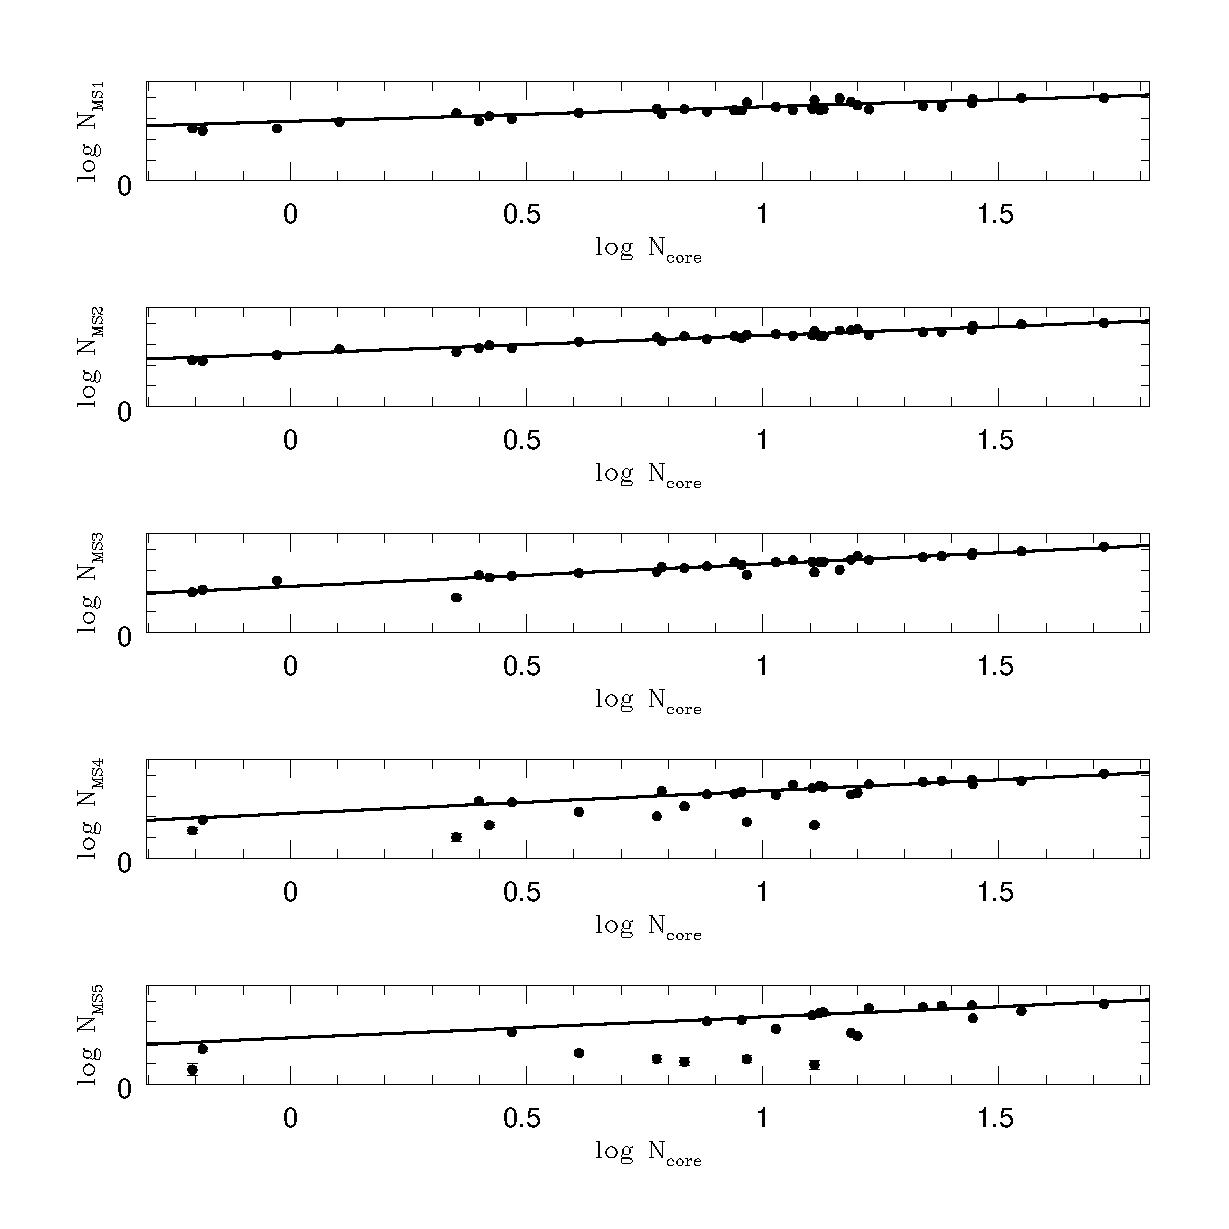
\includegraphics[scale=0.5]{Chapter-6/Ncore_vs_Nms_rc_new.ps}
\caption[Logarithm of the number of
stars belonging to each mass bin as a function of the
logarithm of the total number of stars spanning all five mass
bins in the core]{The logarithm of the number of
stars belonging to each mass bin as a function of the
logarithm of the total number of stars spanning all five mass
bins in the core.  MS1 corresponds to the mass range 0.65 - 0.75 M$_{\odot}$, MS2
to 0.55 - 0.65 M$_{\odot}$, MS3 to 0.45 - 0.55 M$_{\odot}$, MS4 to
0.35 - 0.45 M$_{\odot}$, and MS5 to 0.25 - 0.35 M$_{\odot}$.  Lines of
best fit are shown for each mass bin. 
\label{fig:Ncore_vs_Nms_rc}}
\end{center}
\end{figure}

\begin{figure} [!h]
  \begin{center}
 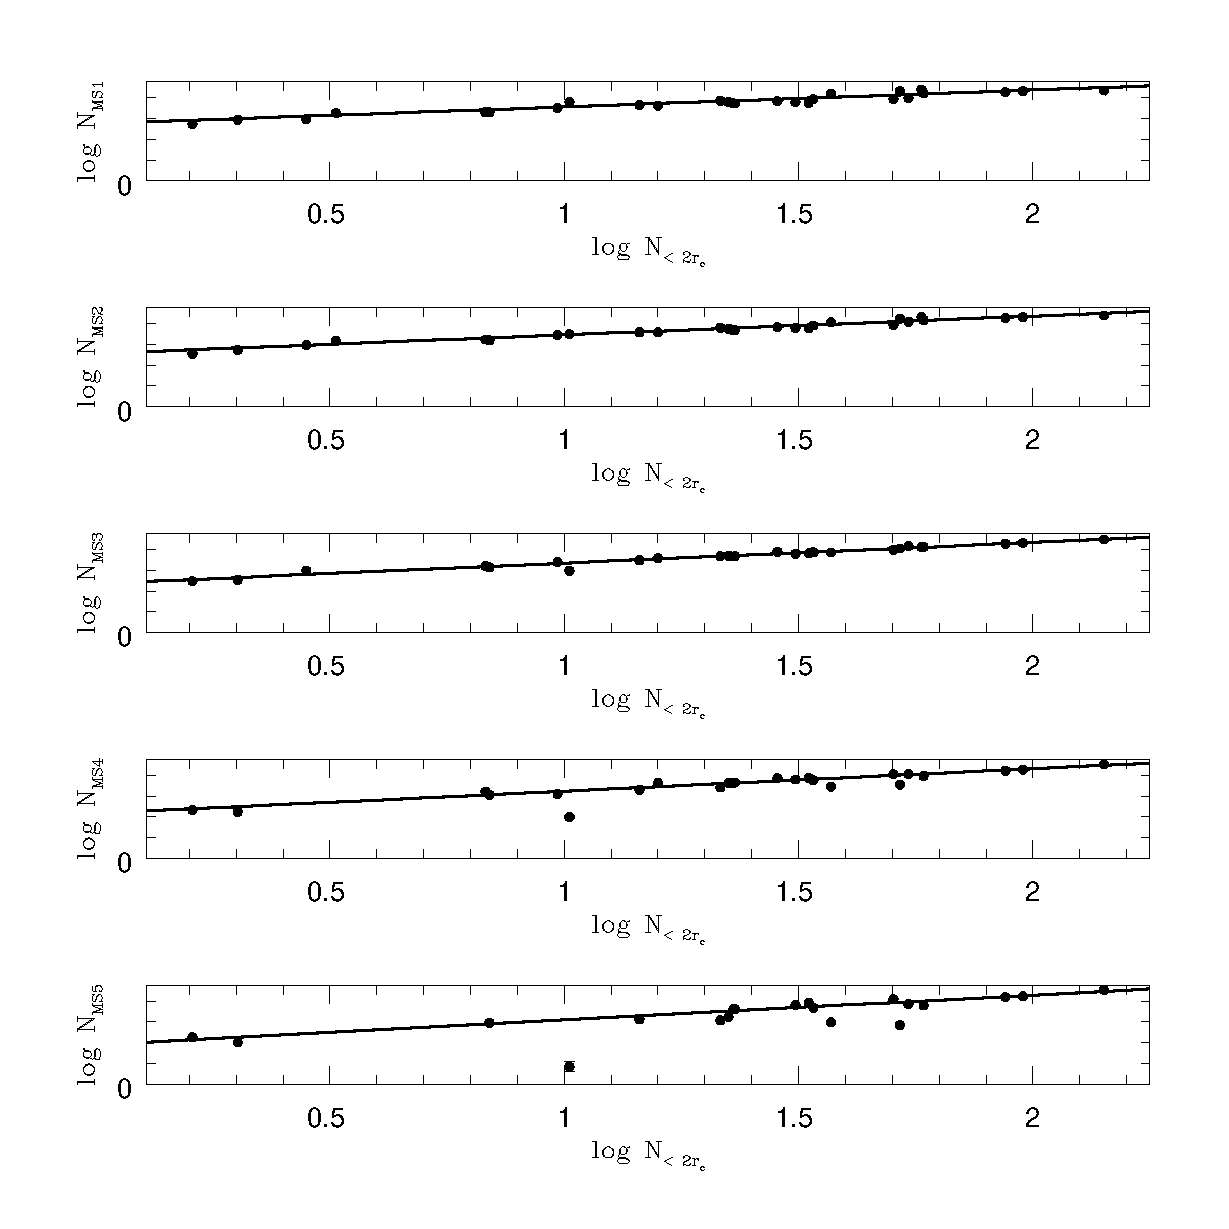
\includegraphics[scale=0.5]{Chapter-6/Ncore_vs_Nms_2rc_new.ps}
\caption[Logarithm of the number of
stars belonging to each mass bin as a function of the
logarithm of the total number of stars spanning all five mass
bins within two core radii from the cluster centre]{The logarithm of the number of
stars belonging to each mass bin as a function of the
logarithm of the total number of stars spanning all five mass
bins within two core radii from the cluster centre.  The mass bins are
the same as in Figure~\ref{fig:Ncore_vs_Nms_rc}.
%MS1 corresponds
%to the mass range 0.65 - 0.75 M$_{\odot}$, MS2
%to 0.55 - 0.65 M$_{\odot}$, MS3 to 0.45 - 0.55 M$_{\odot}$, MS4 to
%0.35 - 0.45 M$_{\odot}$, and MS5 to 0.25 - 0.35 M$_{\odot}$.  Lines of
%best fit are shown for each mass bin.
\label{fig:Ncore_vs_Nms_2rc}}
\end{center}
\end{figure}

\begin{figure} [!h]
  \begin{center}
 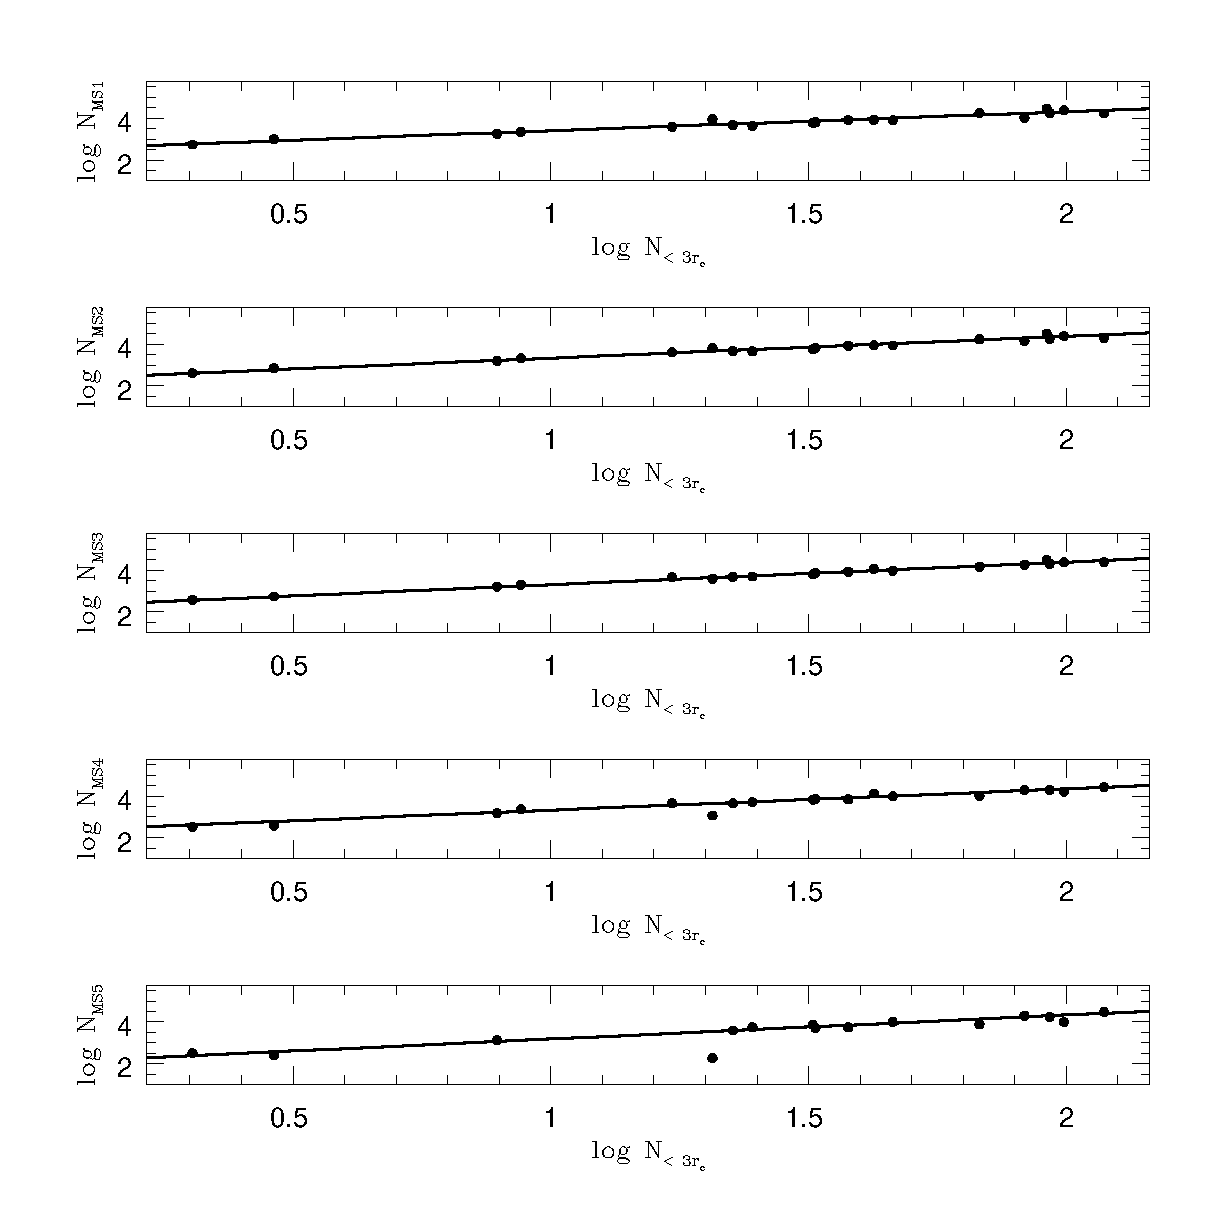
\includegraphics[scale=0.5]{Chapter-6/Ncore_vs_Nms_3rc_new.ps}
 \caption[Logarithm of the number of
 stars belonging to each mass bin as a function of the
 logarithm of the total number of stars spanning all five mass
 bins within three core radii from the cluster centre]{The logarithm of
  the number of
stars belonging to each mass bin as a function of the
logarithm of the total number of stars spanning all five mass
bins within three core radii from the cluster centre.  The mass bins are
the same as in Figure~\ref{fig:Ncore_vs_Nms_rc}.
%MS1 corresponds
%to the mass range 0.65 - 0.75 M$_{\odot}$, MS2
%to 0.55 - 0.65 M$_{\odot}$, MS3 to 0.45 - 0.55 M$_{\odot}$, MS4 to
%0.35 - 0.45 M$_{\odot}$, and MS5 to 0.25 - 0.35 M$_{\odot}$.  Lines of
%best fit are shown for each mass bin.
\label{fig:Ncore_vs_Nms_3rc}}
\end{center}
\end{figure}

%\begin{footnotesize}
\begin{sidewaystable}
\tiny
\centering
\caption{Lines of Best Fit for log N$_{MS}$ = (a $\pm$ $\Delta$a)log (N$_{tot}$/10$^3$) + (b $\pm$ $\Delta$b)
  \label{table:bestfit6}}
%\begin{tabular}{|l|p{4.5cm}|p{3.5cm}|p{3.5cm}|p{3.5cm}|p{3.5cm}|}
\begin{tabular}{|l|cccc|cccc|cccc|cccc|cccc|}
\hline
      &\multicolumn{4}{c|}{   MS1 (0.65-0.75 M$_{\odot}$)  }&\multicolumn{4}{c|}{   MS2 (0.55-0.65 M$_{\odot}$)  }&\multicolumn{4}{c|}{   MS3 (0.45-0.55 M$_{\odot}$)  }&\multicolumn{4}{c|}{   MS4 (0.35-0.45 M$_{\odot}$)  }&\multicolumn{4}{c|}{   MS5 (0.25-0.35 M$_{\odot}$)  }\\
%Circle      &   MS1 (0.65-0.75 M$_{\odot}$)  &   MS2 (0.55-0.65 M$_{\odot}$)  &   MS3 (0.45-0.55 M$_{\odot}$)  &   MS4 (0.35-0.45 M$_{\odot}$)  &   MS5 (0.25-0.35 M$_{\odot}$)  \\
\hline
Circle & a & $\Delta$a & b & $\Delta$b & a &$\Delta$a & b & $\Delta$b
& a & $\Delta$a & b & $\Delta$b & a & $\Delta$a & b & $\Delta$b & a &
$\Delta$a & b & $\Delta$b \\
%Circle       &          MS1 (0.65-0.75 M$_{\odot}$)             &           MS2 (0.55-0.65 M$_{\odot}$)            &              MS3 (0.45-0.55 M$_{\odot}$)            &            MS4 (0.35-0.45 M$_{\odot}$)           &           MS5 (0.25-0.35 M$_{\odot}$)            \\
\hline
$<$ r$_c$    & 0.70 & 0.07 & 2.85 & 0.09 & 0.86 & 0.05 & 2.56 & 0.05 & 1.08 & 0.05 & 2.22 & 0.07 & 1.08 & 0.09 & 2.17 & 0.12 & 1.00 & 0.20 & 2.24 & 0.25 \\
$<$ 2r$_c$   & 0.81 & 0.08 & 2.74 & 0.12 & 0.90 & 0.06 & 2.55 & 0.09 & 0.99 & 0.03 & 2.35 & 0.05 & 1.07 & 0.06 & 2.17 & 0.10 & 1.19 & 0.10 & 1.91 & 0.18 \\
$<$ 3r$_c$   & 0.91 & 0.12 & 2.50 & 0.19 & 1.04 & 0.11 & 2.30 & 0.17 & 1.08 & 0.08 & 2.23 & 0.12 & 1.02 & 0.05 & 2.31 & 0.10 & 1.15 & 0.10 & 2.04 & 0.16 \\
%
%$<$ r$_c$    & log(N$_{MS1}$) = (0.70 $\pm$ 0.07)log(N$_{tot}$/10$^3$) + (2.85 $\pm$ 0.09)  &    log(N$_{MS2}$) = (0.86 $\pm$ 0.05)log(N$_{tot}$/10$^3$) + (2.56 $\pm$ 0.05)    & log(N$_{MS3}$) = (1.08 $\pm$ 0.05)log(N$_{tot}$/10$^3$) + (2.22 $\pm$ 0.07)   & log(N$_{MS4}$) = (1.08 $\pm$ 0.09)log(N$_{tot}$/10$^3$) + (2.17 $\pm$ 0.12)  & log(N$_{MS5}$) = (1.00 $\pm$ 0.20)log(N$_{tot}$/10$^3$) + (2.24 $\pm$ 0.25)  \\
%$<$ 2r$_c$   & log(N$_{MS1}$) = (0.81 $\pm$ 0.08)log(N$_{tot}$/10$^3$) + (2.74 $\pm$ 0.12)  &    log(N$_{MS2}$) = (0.90 $\pm$ 0.06)log(N$_{tot}$/10$^3$) + (2.55 $\pm$ 0.09)    & log(N$_{MS3}$) = (0.99 $\pm$ 0.03)log(N$_{tot}$/10$^3$) + (2.35 $\pm$ 0.05)   & log(N$_{MS4}$) = (1.07 $\pm$ 0.06)log(N$_{tot}$/10$^3$) + (2.17 $\pm$ 0.10)  & log(N$_{MS5}$) = (1.19 $\pm$ 0.10)log(N$_{tot}$/10$^3$) + (1.91 $\pm$ 0.18)  \\
%$<$ 3r$_c$   & log(N$_{MS1}$) = (0.91 $\pm$ 0.12)log(N$_{tot}$/10$^3$) + (2.50 $\pm$ 0.19)  &    log(N$_{MS2}$) = (1.04 $\pm$ 0.11)log(N$_{tot}$/10$^3$) + (2.30 $\pm$ 0.17)    & log(N$_{MS3}$) = (1.08 $\pm$ 0.08)log(N$_{tot}$/10$^3$) + (2.23 $\pm$ 0.12)   & log(N$_{MS4}$) = (1.02 $\pm$ 0.05)log(N$_{tot}$/10$^3$) + (2.31 $\pm$ 0.10)  & log(N$_{MS5}$) = (1.15 $\pm$ 0.10)log(N$_{tot}$/10$^3$) + (2.04 $\pm$ 0.16)  \\
\hline
\end{tabular}
\end{sidewaystable}

As shown in Table~\ref{table:bestfit6}, the slopes tend to
systematically increase 
with decreasing mass bin.  For the comparison within two core radii
(shown in Figure~\ref{fig:Ncore_vs_Nms_2rc}), 
this trend applies to all mass bins.  For the comparisons within the core
and within three core radii (shown in Figure~\ref{fig:Ncore_vs_Nms_rc}
and Figure~\ref{fig:Ncore_vs_Nms_3rc}, respectively), however, only
the highest three mass bins (MS1, MS2, and MS3) 
follow this trend of increasing slope with decreasing mass bin.  After
the third mass bin, the slopes for the lowest two mass bins remain
about the same.  Note, however, that the uncertainties on the slopes
and y-intercepts are also higher for the lowest mass bins (MS4 and MS5).  
%
%For the most part, the slopes for each mass bin are consistent with their
%adjacent bins to within one standard deviation.  This is particularly
%true for the lowest two mass bins (MS4 and MS5) for which the
%uncertainties are typically the largest.  
This is
likely to be due to the fact that the photometric errors are the
highest at these dim magnitudes, however they remain at most $\sim$
10\% of the width in magnitude of their corresponding mass bins.  The
completeness corrections are also the largest for MS4 and MS5,
and this also introduces additional uncertainty.  Although we have
taken the appropriate measures, it
is important that these effects be properly quantified in order to reliably
use our technique to constrain the degree of universality of the IMF.
We will return to this in Section~\ref{discussion6}.  

On the other hand, when we consider only the largest three mass bins
(MS1, MS2, and MS3) for which 
the photometric errors and level of incompleteness are the lowest, the
difference in slopes and y-intercepts between adjacent mass bins can
differ at better than the $2-\sigma$ confidence level.  Moreover, if we
compare non-adjacent mass bins, then this trend is typically
significant at the $3-\sigma$ confidence level.  In order to improve
upon these statistics, we have also calculated reduced chi-squared
values with added intrinsic dispersion for the relations for each mass
bin.  That is, for each mass bin we added a constant term to the uncertainty for each
data point, found the value that yielded a reduced chi-squared of one,
and looked at the subsequent effects on the uncertainties for the
line of best-fit.  Based on this, we appear to be slightly over-estimating the
uncertainties for the MS1, MS2 and MS3 mass bins using our bootstrap
approach, and slightly under-estimating them for the MS4 and MS5
bins.  This suggests that the slopes and y-intercepts differ at nearly
the $2-\sigma$ confidence level for the MS1, MS2 and MS3 mass bins,
but are consistent to within one standard deviation for the MS4 and
MS5 bins.  We conclude that our results are the most reliable (at nearly the
$2-\sigma$ confidence level) in the mass range 0.45-0.75 M$_{\odot}$. 

The change in the distribution of stellar masses as a function of the
total cluster mass can be illustrated using pie charts, as shown in
Figure~\ref{fig:pie_charts}.  Using the slopes and y-intercepts
provided in Table~\ref{table:bestfit6} for the comparison within two core
radii, we have generated pie charts for three total numbers of stars
(spanning all five mass bins), namely N$_{tot}$ = 10$^3$, 10$^4$,
10$^5$.  As is clear, low-mass stars are preferentially depleted, and
this effect becomes increasingly severe with decreasing total cluster
mass (or, equivalently, increasing dynamical age).  From right to
left, what the pie charts are showing are the mass
functions of progressively dynamically older clusters.  %We will
%return to this issue in Section~\ref{discussion6}.  
If this is indeed the cause of the observed depletion of low-mass
stars in low-mass clusters, we are effectively looking at the
evolution of the stellar mass function in time.   

\begin{figure} [!h]
  \begin{center}
 \includegraphics[scale=0.5]{Chapter-6/pie_charts.ps}
    \caption[Mass Functions in Pie Chart Form]{
      Stellar mass functions depicted in pie chart form.  The total
      area of each circle corresponds to the total number of stars
      spanning all five mass bins, and each pie slice shows the
      fraction of this total corresponding to each mass bin.  Each of
      these fractions was calculated using the weighted lines of
      best-fit provided in Table~\ref{table:bestfit6}.  From left to
      right, the total number of stars used to generate each pie chart
      was 10$^3$, 10$^4$, and 10$^5$.  Dark blue corresponds to MS1,
      red to MS2, green to MS3, purple to MS4, and light blue to MS5.
      From right to left, the pie charts effectively show the mass functions of
      progressively dynamically older clusters.
      \label{fig:pie_charts}}
    \end{center}
\end{figure}

\section{Summary \& Discussion} \label{discussion6}

In this chapter, we have obtained completeness-corrected stellar mass
functions in the range 0.25-0.75 M$_{\odot}$ for a sample of 33
globular clusters using data taken from the ACS Survey for Globular
Clusters.  We have presented a new technique to quantify
cluster-to-cluster variations in the observed stellar mass functions.  
We have shown how our method can be used to quantify the universality
of the IMF for a large sample of clusters and, when used in
conjunction with theoretical models for globular cluster evolution,
can be used to constrain the degree to which two-body relaxation has
modified the currently observed stellar mass functions from their 
primordial form.  To this end, we have
obtained weighted lines of best-fit by comparing the number of stars in five
different mass bins to the total number of stars spanning the
entire mass range within several circles centred on the cluster
centre.  

As shown in Table~\ref{table:bestfit6}, our results suggest that the slopes
for the lines of best-fit tend to systematically increase
with decreasing mass bin.  Assuming all of the clusters in our sample
were born with similar IMFs, this is precisely what we expect from
two-body relaxation.  That is, we expect low-mass stars to become
preferentially depleted via stellar evaporation, and we expect this
effect to be the most severe in low-mass clusters.  This trend is
clearly seen in the observations, as demonstrated in 
Figure~\ref{fig:pie_charts}.  Interestingly, the fraction of stars
belonging to each mass bin is remarkably constant for all mass bins at
the high-mass end of our sample.  The total masses of these clusters
are sufficiently high that their half-mass relaxation times are
comparable to their ages \citep[e.g.][]{harris96}.  Therefore, we
expect that the highest mass clusters in our sample should have
been relatively unaffected by stellar evaporation due to two-body
relaxation.  It follows that their current mass functions should be
relatively unchanged from their primordial values (ignoring the
effects of stellar evolution).  If true, our
results could suggest that the slope IMF in Equation~\ref{eqn:kroupa}
was consistent with zero in the
mass range 0.25-0.75 M$_{\odot}$ for all of the clusters in our
sample.  This would be inconsistent with a ``standard'' Kroupa IMF.  This
hypothesis can be tested by comparing the results of the 
observational analysis presented in this chapter to simulations of
globular cluster evolution.  These can be used to directly quantify
the effects of two-body relaxation on the expected slopes and
y-intercepts for each mass bin given any set of initial conditions and
IMFs.  By comparing the results of these simulations to the results of
our observational analysis, the set of initial conditions that
best reproduces the observations can be found.  This will tell us
about the precise functional form of the IMF for the clusters in our
sample, in addition to the degree of primordial mass segregation.

The uncertainties for the slopes and 
y-intercepts are sufficiently large that they are often consistent with
those of their adjacent mass bins to within one standard deviation.
However, when we consider only the largest three mass bins for which
the photometric errors and level of incompleteness are the lowest, the
difference in slopes and y-intercepts between adjacent mass bins can
differ at better than the $2-\sigma$ confidence level.  Moreover, the
trend of increasing slope with decreasing mass is typically
significant at the $3-\sigma$ confidence level if we compare
non-adjacent mass bins.  Based on this, we conclude that our results
are consistent with a universal IMF for the clusters in our sample,
and that the currently observed mass functions have primarily been 
modified by internal two-body relaxation.  Having said that, it is
important to note that a higher degree of primordial mass segregation
effectively acts
to increase the rate of dynamical evolution and therefore stellar
evaporation \citep[e.g.][]{heggie03}.  Consequently, our results could
also be consistent with a non-universal IMF that depends on the total
cluster mass, provided the degree of primordial mass segregation also
depends systematically on the total cluster mass.  We also wish to
point out here 
that the large uncertainties found for the slopes and y-intercepts,
particularly for the two lowest mass bins, are primarily due to the
relatively large photometric errors at these dim magnitudes and
incompleteness resulting from crowding.  Despite the high quality of
the data used in this study, these issues are currently unavoidable
given the nature of the observations.  This will be a key challenge
for future studies to resolve, however the method we have presented
in this chapter offers a robust means of performing future analyses.

In terms of addressing the \textit{degree} of universality of the IMF,
our technique offers a considerable advantage over the standard
power-law and log-normal forms used to characterize the stellar mass
function shown in Equation~\ref{eqn:kroupa} and
Equation~\ref{eqn:miller}.  This is the case when comparing the mass
functions of a large sample of clusters.  The reason for this is that
our method
segments the mass function into mass bins, which characterizes
cluster-to-cluster differences in the stellar mass function for each
mass bin individually (i.e. as a function of stellar mass).  This
is done using the slopes and y-intercepts of the
relations found by correlating the number of stars in each mass bin
with the total number of stars spanning all mass bins.  Conversely,
standard Kroupa or Chabrier mass functions quantify the mass function
much more globally via functional fits to the data over considerably
larger mass ranges.  Of course, the standard forms
remain as useful as ever for characterizing the mass functions of
individual clusters, whereas our method is not appropriate for
this purpose.  That being
said, it is worth stating here that our results 
are consistent with those of \citet{demarchi10}, who fit a tapered
power-law distribution function with an exponential truncation to the
stellar mass functions of a sample of 30 clusters containing both
young and old members. 

There are several possible sources of additional uncertainty that
could have affected our analysis.  For 
instance, we have not yet considered the role played by binaries.
These tend to be unresolved in GCs, usually appearing as single
objects located above the MS in the 
cluster CMD.  Therefore, some of the objects in each mass bin are in
fact binaries masquerading as single stars.  Typical binary fractions
in Milky Way GCs are thought to be on the order of a few to a few tens
of a percent \citep[e.g.][]{rubenstein97, cool02, sollima08,
  davis08}.  This suggests that a non-negligible number of binaries
could often be included in our number counts for each mass bin.
However, there is no reason not to expect that binaries will
contribute to each mass bin in 
roughly equal proportions.  If the fraction of binaries is the same in
all mass bins, then the presence of binaries should not have
significantly affected the slopes.  Although they will have
affected the y-intercepts, this effect should not cause them to deviate
from within the uncertainties and 
should not have affected the interpretation of our results.  On the 
other hand, some observational evidence suggests that
the binary fraction could be inversely proportional to the total
cluster mass \citep[e.g.][]{sollima08, milone08, knigge09}.  It is not
clear how this might have affected our results since we do not know
how each mass bin should be affected.  It is our intent to address
this issue in a future study once binary fractions become available for
the majority of the clusters in our sample (Ata Sarajedini; private
communication).

Throughout our analysis, we have 
consistently compared two projected quantities.  Therefore, effects
related to projection should not have significantly affected
our results.  Moreover, these effects should become less severe upon
considering progressively larger circles, and we have performed 
our analysis for circles with three different sizes.  We note that
this could perhaps help to explain why 
the scatter in the lowest mass bins appears to become reduced for the
comparisons within two and three core radii (compared to the
comparison within one core radius), although it is not clear
why the agreement appears slightly better for the former comparison.  

Tidal effects from the Galaxy effectively act to reduce the time-scale
for two-body relaxation \citep[e.g.][]{heggie03}.  The same effect can also be had by
increasing the degree of primordial mass segregation
\citep[e.g.][]{spitzer87, portegieszwart01}.  Therefore, on average,
we would expect clusters with smaller Galactocentric radii and higher
initial concentrations to have experienced a higher degree of stellar
evaporation.  In an effort to quantify tidal effects from the Galaxy,
we performed several cuts in perigalacticon distance \citep{dinescu99,
  dinescu07} and re-performed our weighted lines of best-fit.  Despite
removing clusters from our sample with small perigalacticon distances
for which it is typically argued that tidal effects should be the most
severe \citep[e.g.][]{heggie03}, our slopes and 
y-intercepts, in addition to their uncertainties, remain more or less
unchanged.  This can be interpreted as rough evidence that tidal effects
from the Galaxy have not 
significantly affected our results.  It is much less clear which
clusters in our sample, if any, were born with high central 
concentrations.  Based on current observations, there is no
known reason not to expect a universal degree of primordial mass
segregation \citep[e.g.][]{portegieszwart10}.  If this was the case,
then our results could be interpreted as indicative of a
universal IMF for Milky Way globular clusters.  Unfortunately,
observational constraints for primordial 
binary populations are also lacking \citep[e.g.][]{mckee07}.  Binaries
play an important 
role in star cluster evolution by, for instance, providing an energy
source that serves to resist a cluster's tendency toward increasing 
its central density \citep{hut83}.  They are therefore an important consideration in
deciding the dynamical evolution of the stellar mass function, and
their role will need to be addressed in future studies.  

It is interesting and even surprising that, despite all of the
aforementioned factors 
expected to affect the dynamical evolution of globular clusters, we
observe relatively little scatter in the relations within two and
three core radii (Figure~\ref{fig:Ncore_vs_Nms_2rc} and
Figure~\ref{fig:Ncore_vs_Nms_3rc}).  Moreover, the slopes
systematically increase with decreasing mass bin.  Based on this, our
results are consistent with a single universal IMF for all of the
clusters in our sample that has been modified via internal two-body
relaxation by an amount determined by the total cluster mass.  
%and external effects such as tides from the Galaxy play a much less
%significant role (or that they are comparable in all clusters).
%Our results could also suggest that the initial cluster 
%conditions, including primordial mass segregation and the primordial
%binary fraction, are approximately universal for all Galactic GCs. 
%
%The small degree of scatter observed in
%Figure~\ref{fig:Ncore_vs_Nms_2rc} and
%Figure~\ref{fig:Ncore_vs_Nms_3rc} 
%Finally, our results provide compelling evidence of an approximately 
%universal IMF among all Galactic globular clusters.  
%The evidence in favour of a universal IMF is particularly compelling.
%Based on our results, this holds true for old Milky Way globular clusters
%having metallicities in the range [Fe/H] $\sim$ -(0.37 - 2.28)
%\citep{dotter10}.  
This is a new result given 
the old ages and therefore low metallicities ([Fe/H] $\sim$ -2.28 -
(-0.37)) of the clusters that comprise our sample.  However, the  
exact form of the IMF required to reproduce the current observations is
still not clear, nor is the role of primordial mass segregation.  To
what degree have low-mass clusters been depleted of 
their low-mass stars?  What combination of IMFs, Galactocentric
radii, initial concentrations and primordial binary fractions 
should evolve dynamically to best reproduce the currently observed
mass functions?  These questions can only be answered using 
simulations of globular cluster evolution that explore a range of
initial conditions and IMFs.  Our observational analysis of
the ACS data is ideally suited for comparison to these types of
models.  This would allow us to constrain the precise shape of the IMF
in the mass and metallicity range of interest, as well as to learn about
primordial mass segregation.  This will be the focus of a forthcoming
study. 

%
%PHOTOMETRIC ERRORS AND COMPLETENESS - both worse for dim, low-mass
%stars in the lowest two mass bins, hence the higher uncertainties.

\section*{Acknowledgments}

We would like to thank Ata Sarajedini, Aaron Dotter and Roger Cohen
for providing the data on which this study is based and for their
extensive support in its analysis.  We would also like to thank Evert
Glebbeek for useful discussions.  This research has been
supported by NSERC and OGS.

%\chapterbib

\begin{thebibliography}{99}

\bibitem[\protect\citeauthoryear{Anderson et al.}{2008}]{anderson08}
  Anderson J.,  Sarajedini A., Bedin L. R., King I. R., Piotto G.,
  Reid I. N., Siegel M., Majewski S. R., Paust N. E. Q., Aparicio A.,
  Milone A. P., Chaboyer B., Rosenberg A. 2008, AJ, 135, 2055
\bibitem[\protect\citeauthoryear{Bonnell, Larson \&
    Zinnecker}{2007}]{bonnell07} Bonnell I. A., Larson R. B.,
  Zinnecker H. 2007, Protostars and Planets V, 149 
  Elmegreen B. G. 1999, ApJ, 527, 266
\bibitem[\protect\citeauthoryear{Chabrier}{2005}]{chabrier05} Chabrier
  G. 2005, ASSL Vol. 327: The Initial Mass Function 50 Years Later, 41
\bibitem[\protect\citeauthoryear{Cool et al.}{2002}]{cool02} Cool
  A. M., Bolton
  A. S. 2002, in ASP Conference Series 263, Stellar Collisions,
  Mergers and their Consequences, ed. M. M. Shara (San Francisco:
  ASP), 163
\bibitem[\protect\citeauthoryear{Da Costa}{1982}]{dacosta82} Da Costa
  G. S. 1982, AJ, 87, 990
\bibitem[\protect\citeauthoryear{Davis et al.}{2008}]{davis08}
  Davis D. S., Richer H. B., Anderson J., Brewer J., Hurley J.,
  Kalirai J. S., Rich R. M., Stetson P. B. 2008, AJ, 135, 2155
\bibitem[\protect\citeauthoryear{Dinescu, Girard \& van
    Altena}{1999}]{dinescu99}
  Dinescu D. I., Girard T. M., van Altena W. F. 1999, AJ, 117, 1792
\bibitem[\protect\citeauthoryear{Casetti-Dinescu et al.}{2007}]{dinescu07}
  Casetti-Dinescu D. I., Girard T. M., Herrera D., van Altena W. F.,
  Lopez C. E., Castillo D. J. 2007, AJ, 134, 195
\bibitem[\protect\citeauthoryear{De Angeli et al.}{2005}]{deangeli05}
  De Angeli F., Piotto G., Cassisi S., Busso G., Recio-Blanco A.,
  Salaris M., Aparicio A., Rosenberg A. 2005, AJ, 130, 116
\bibitem[\protect\citeauthoryear{De Marchi, Paresce \& Portegies
    Zwart}{2010}]{demarchi10} De Marchi G., Paresce F., Portegies
  Zwart S. 2010, ApJ, 718, 105
\bibitem[\protect\citeauthoryear{Dotter et al.}{2007}]{dotter07}
  Dotter A., Chaboyer B., Jevremovic D., Baron E., Ferguson J. W.,
  Sarajedini A., Anderson J. 2007, AJ, 134, 376
\bibitem[\protect\citeauthoryear{Dotter et al.}{2010}]{dotter10}
  Dotter, A., Sarajedini A., Anderson J., Aparicio A., Bedin L. R.,
  Chaboyer B., Majewski S., Marin-Franch A., Milone A., Paust N.,
  Piotto G., Reid  N., Rosenberg A., Siegel M. 2010, ApJ, 708, 698
\bibitem[\protect\citeauthoryear{Elmegreen}{1999}]{elmegreen99}
  Elmegreen B. G. 1999, ApJ, 527, 266
\bibitem[\protect\citeauthoryear{Elmegreen}{2001}]{elmegreen01}
  Elmegreen B. G. 2001, ASP Conference Series 243: From Darkness to Light:
  Origin and Evolution of Young Stellar Clusters, 243, 255
\bibitem[\protect\citeauthoryear{Gieles et al.}{2010}]{gieles10}
  Gieles M., Baumgardt H., Heggie D., Lamers H. 2010, MNRAS, 408, L16
\bibitem[\protect\citeauthoryear{Gieles, Heggie \&
    Zhao}{2011}]{gieles11} Gieles M., Heggie D., Zhao H. 2011, MNRAS,
  accepted 
\bibitem[\protect\citeauthoryear{Goldsbury et al.}{2010}]{goldsbury10}
  Goldsbury R., Richer H. B., Anderson J., Dotter A., Sarajedini A.,
  Woodley K. 2010, AJ, 140, 1830
\bibitem[\protect\citeauthoryear{Grenier, Casandijan \&
    Terrier}{2005}]{grenier05} Grenier I. A., Casandjian J. M.,
  Terrier R. 2005, Science, 307, 1292
\bibitem[\protect\citeauthoryear{Harris}{1996, 2010 update}]{harris96}
  Harris, W. E. 1996, AJ, 112, 1487 (2010 update)
\bibitem[\protect\citeauthoryear{Heggie \& Hut}{2003}]{heggie03}
  Heggie D. C., Hut P. 2003, The Gravitational Million-Body Problem:
  A Multidisciplinary Approach to Star Cluster Dynamics (Cambridge:
  Cambridge University Press)
\bibitem[\protect\citeauthoryear{Henon}{1960}]{henon60} Henon M. 1960,
  Annales d'Astrophysique, 23, 668
\bibitem[\protect\citeauthoryear{Henon}{1973}]{henon73} Henon
  M. 1973, Dynamical Structure and Evolution of Dense Stellar Systems,
  ed. L. Martinet \& M. Mayor (Geneva Obs.)
\bibitem[\protect\citeauthoryear{Hurley et al.}{2005}]{hurley05}
  Hurley, J. R., Pols, O. R., Aarseth, S. J. \& Tout, C. A. 2005,
  MNRAS, 363, 293
\bibitem[\protect\citeauthoryear{Hut}{1983}]{hut83} Hut P. 1983, ApJ,
  272, 29
\bibitem[\protect\citeauthoryear{Knigge, Leigh \&
    Sills}{2009}]{knigge09} Knigge C., Leigh
  N., Sills A. 2009, Nature, 457, 288
\bibitem[\protect\citeauthoryear{Kroupa}{2001}]{kroupa01} Kroupa
  P. 2001, MNRAS, 322, 231
\bibitem[\protect\citeauthoryear{Lada}{1985}]{lada85} Lada C. J. 1985,
  ARA\&A, 23, 267
\bibitem[\protect\citeauthoryear{Lada \& Lada}{1995}]{lada95} Lada
  E. A., Lada C. J. 1995, AJ, 109, 1682
\bibitem[\protect\citeauthoryear{Lada \& Lada}{2003}]{lada03} Lada
  C. J., Lada E. A. 2003, ARA\&A, 41, 57
\bibitem[\protect\citeauthoryear{Lada, Alves \&
    Lombardi}{2007}]{lada07} Lada C. J., Alves J. F., Lombardi
  M. 2007, Protostars and Planets V, 3
\bibitem[\protect\citeauthoryear{McKee \& Ostriker}{2007}]{mckee07}
  McKee C. F., Ostriker E. C. 2007, ARA\&A, 45, 565
\bibitem[\protect\citeauthoryear{Miller \& Scalo}{1979}]{miller79}
  Miller G. E., Scalo J. M. 1979, ApJS, 41, 513
\bibitem[\protect\citeauthoryear{Milone et al.}{2008}]{milone08}
  Milone A. P., Piotto G., Bedin L. R., Sarajedini A. 2008, MmSAI, 79,
  623
\bibitem[\protect\citeauthoryear{Murray}{2009}]{murray09} Murray
  N. 2009, ApJ, 691, 946
\bibitem[\protect\citeauthoryear{Portegies Zwart et
    al.}{2001}]{portegieszwart01} Portegies Zwart S. F., McMillan
  S. L. W., Hut P., Makino J. 2001, MNRAS, 321, 199
\bibitem[\protect\citeauthoryear{Portegies Zwart, McMillan \&
    Gieles}{2010}]{portegieszwart10} Portegies Zwart S. F., McMillan
  S. L. W., Gieles M. 2010, ARA\&A, 48, 431
\bibitem[\protect\citeauthoryear{Rubenstein \&
    Bailyn}{1997}]{rubenstein97} Rubenstein E. P., Bailyn C. D. 1997,
  ApJ, 474, 701
\bibitem[\protect\citeauthoryear{Sarajedini et
    al.}{2007}]{sarajedini07}
  Sarajedini A., Bedin L. R., Chaboyer B., Dotter  A., Siegel M.,
  Anderson J., Aparicio A., King I., Majewski S., Marin-Franch A.,
  Piotto G., Reid  I. N., Rosenberg A., Steven M. 2007, AJ, 133, 1658
\bibitem[\protect\citeauthoryear{Scalo}{1998}]{scalo98} Scalo J. 1998,
  ASP Conference Series 142: The Stellar Initial Mass Function (38th
  Herstmonceux Conference), 142, 201
\bibitem[\protect\citeauthoryear{Sollima et al.}{2007}]{sollima07}
  Sollima A., Beccari G., Ferraro F. R., Fusi Pecci F., Sarajedini
  A. 2008, MNRAS, 380, 781
\bibitem[\protect\citeauthoryear{Sollima et al.}{2008}]{sollima08}
  Sollima A., Beccari G., Ferraro F. R., Fusi Pecci F., Sarajedini
  A. 2007, A\&A, 481, 701
\bibitem[\protect\citeauthoryear{Spitzer}{1987}]{spitzer87} Spitzer
  L. 1987, Dynamical Evolution of Globular Clusters (Princeton:
  Princeton University Press)
\bibitem[\protect\citeauthoryear{von Hippel \&
    Sarajedini}{1998}]{vonhippel98} von Hippel T., Sarajedini A. 1998,
  AJ, 116, 1789

\end{thebibliography}

%\bsp

%\label{lastpage}

%\end{document}
